\newpage
\section{Durchführung}
    \subsection{Versuchsaufbau}
        Der Aufbau zur Untersuchung von Oberflächen mit Hilfe von Röntgenreflekometrie setzt sich aus drei Hauptbestandteilen zusammen, die den in Abbildung \ref{fig:D8} dargestellten komerziellen 
        Röntgenreflekometrie-Aufbau \textit{D8} bilden. Die Quelle der Röntgenstrahlung stellt eine Röntgenröhre mit Kupferanoden dar und ist 
        wie der Detektor um den Probentisch rotierbar. Die Röntgenröhre wird mit einer Beschleunigungsspannung von \SI{40}{\kilo\electronvolt} betrieben und sendet zunächst einen divergierenden Strahl aus, 
        der das gesamte Röntgenspektrum enthält. Da jedoch nur eine bestimmte Wellenlängenkomponente genutzt werden soll, wird der Strahl auf einen Göbel-Spiegel gerichtet. Dieser kollimiert den Strahl 
        aufgrund seiner parabolischen Form und ist gleichzeitig dazu in der Lage den Strahl zu monochromatisieren. Dies wird über eine Schichtung von Spiegelebenen in definierten Abständen erreicht, sodass
        nur die gewünschte Wellenlänge die Bragg-Bedingung erfüllt und konstruktiv interferiert. Zur Positionierung der Probe wird ein in x-, y- und z-Richtung beweglicher Probentisch genutzt, auf dem die 
        Probe aufliegt. Eine konzeptionelle Darstellung des Aufbaus ist in Abbildung \ref{fig:Aufbau} dargestellt. Alle Komponenten werden über das Programm \textit{XRD Commander} angesteuert und auch die 
        Zählraten des Detektor werdden mit diesem Programm aufgenommen und anschließend ausgewertet.



        \begin{figure}[h]
            \centering
            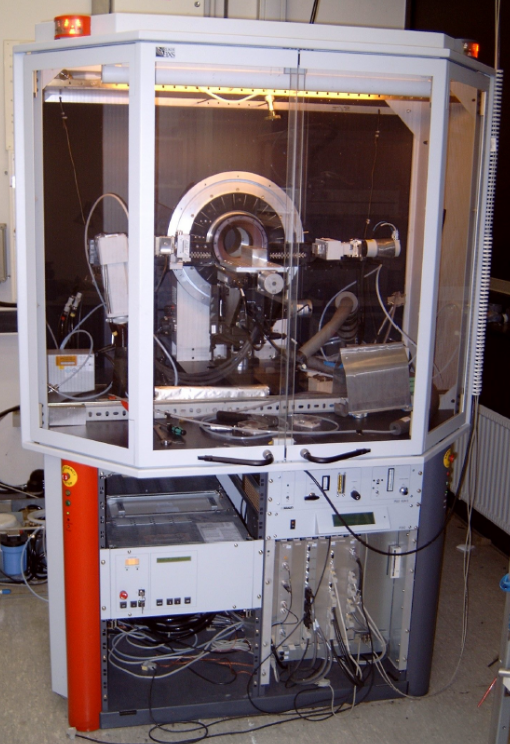
\includegraphics[width = 0.3\textwidth]{pictures/Bild_D8.png}
            \caption{Foto des D8-Laborrefraktometers, das zur Röntgenrefletivitätsmessung genutzt wird. Entnommen aus \cite{tu_dortmund_versuchsanleitung_2022}}
            \label{fig:D8}
        \end{figure}

        \FloatBarrier

        \begin{figure}[h]
          \centering
          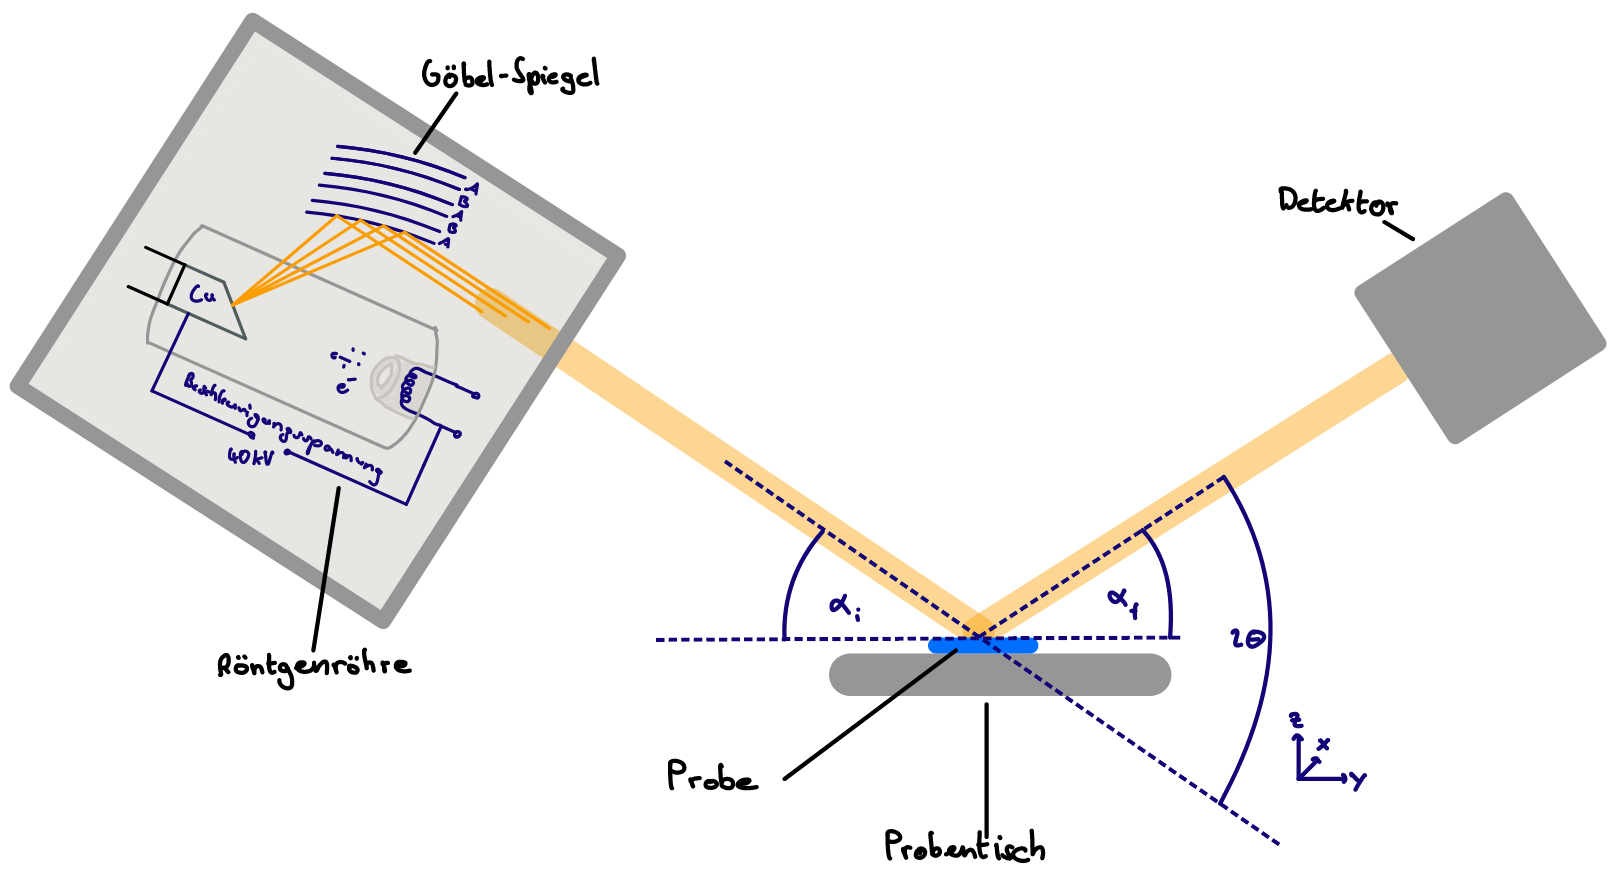
\includegraphics[width = 0.8\textwidth]{pictures/Aufbau.png}
          \caption{Der konzeptionelle Aufbau zur Untersuchung der Probe durch Röntgenreflekometrie. Die Röntgenquelle enthält eine Röntgenröhre und einen Göbelspiegel. Der Probentisch ist in x-, y- und z-Richtung verschiebbar. Zur Variation des $2\theta$-Winkels sind die Röntgenquelle und der Detektor um den Probentisch rotierbar.}
          \label{fig:Aufbau}
        \end{figure}
    
        \FloatBarrier

    

    \subsection{Kalibrierung des Reflektionsaufbaus}
        Um eine optimale Refelektionsmessung durchführen zu können, muss die Probe, wie in Abbildung \ref{fig:parallel} dargestellt zunächst halb in den Strahlengang gefahren sein und exakt parallel zum Strahl 
        liegen, der 
        von der Röntgenquelle zum Detektor läuft, die ebenfalls entlang einer Linie ausgerichtet sein müssen. Um diese Messgeometrie zu garantieren müssen mehrere Scans durchgeführt werden. Diese werden 
        konzeptionell erklärt und die exakten Scan-Parameter in Tabelle \ref{tab:Scan_parameter} aufgelistet.\newline

        \FloatBarrier
        \begin{figure}[h]
            \centering
            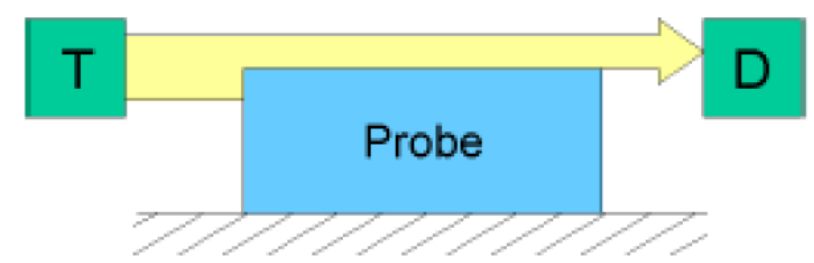
\includegraphics[width = 0.4\textwidth]{pictures/probe_parallel.png}
            \caption{Die zur Justage gewünschte Messgeometrie, bei der die Probe parallel zum Strahl halb in diesem liegt und Röntgenquelle sowie Detektor auf einer Linie liegen. Entnommen aus \cite{tu_dortmund_versuchsanleitung_2022}}
            \label{fig:parallel}
          \end{figure}
      
        \FloatBarrier
  

        Zu Beginn wird die Röntgenröhre auf einen Winkel von $\alpha_{\text{i}} = 0°$ gestellt und die Probe aus dem Strahlengang gefahren. Dann fährt der Detektor in einem \textbf{Detektorscan} einen geringen 
        Winkelbereich um 0° herum ab und misst dabei die Intensität. Dabei sollte sich ein Gauß-Profil ergeben, aus dem der Winkel bestimmt wird, bei dem Röntgenquelle und Detektor genau entlang einer Quelle 
        liegen. Dieser Winkel wird als neue Referenz gesetzt.\newline
        
        Nachem die Probe per Augenmaß in x- und y-Richtung so zentriert wurde, dass sie vom Strahl getroffen wird, wird ein \textbf{z-Scan} durchgeführt. Bei diesem wird die Probe langsam in den Strahlengang 
        gefahren und währenddessen wieder die Intensität gemessen. Aus der resultierenden Kurve, in der die Intensität gegen die z-Koordinate aufgetragen ist, wird die z-Koordinate gewähöt, bei der die Intensität
        auf die halbe maximale Intensität abgesunken ist. Bei dieser Koordinate befindet sich die Probe halb im Strahlengang.\newline
        
        Um die Parallelität der Probe zum Strahl zu garantieren, folgt ein \textbf{Rockingscan}. Die Probe befindet sich in halber Abschattung und Detektor sowie Röntgenquelle erhöhen beziehungsweise verringern 
        ihren Winkel zur Probe, sodass $2\theta$ konstant bleibt. Dies entspricht einer Drehung der Probe im Strahl. Die dabei vermessende Intensität sollte ein Dreieck ergeben, dessen Maximum als $2\theta=0°$
        gewählt wird. Wenn eine der Flanken des Dreiecks stärker fällt als die andere Flanke, muss die y-Position der Probe angepasst werden. Bei einem gleichschekligen Dreieck mit Maximum bei $2\theta=0°$ ist
        die parallel Ausrichtung der Probe zum Strahl erreicht.\newline

        Da die Winkeländerung des Strahlverlaufs die Abschattung des Strahls durch die Probe verändert haben kann, wird ein erneuter \textbf{z-Scan} analog zum Ersten durchgeführt. 

        Anschließend wird ein weiterer \textbf{Rockingscan} bei einem Winkel von $2\theta = \SI{0.3}{\degree}$ durchgeführt, um anschließend anhand eines Intensitätpeaks die Ein- und Ausfallswinkel von 0,15°
        für Röntgenquelle und Detektor zu bestimmen. 

        Um bei der Refelektionsmessung die Probe möglichst komplett mit dem Strahl zu treffen, muss die z-Position auch für einen Winkel von $2\theta\neq0°$ justiert werden. Dazu wird ein Winkel von
        $2\theta = \SI{0.3}{\degree}$ eingestellt und erneut ein \textbf{z-Scan} um die zuvor bestimmte z-Position halber Abschattung durchgeführt. Die Intensitätsmessung soll ein Maximum liefern dessen 
        z-Position als neue Position für die letztendlichen Messungen gewählt wird und die mittlere Geometrie aus Abbildung \ref{fig:zScan_Winkel} garantiert.

        \FloatBarrier
        \begin{figure}[h]
            \centering
            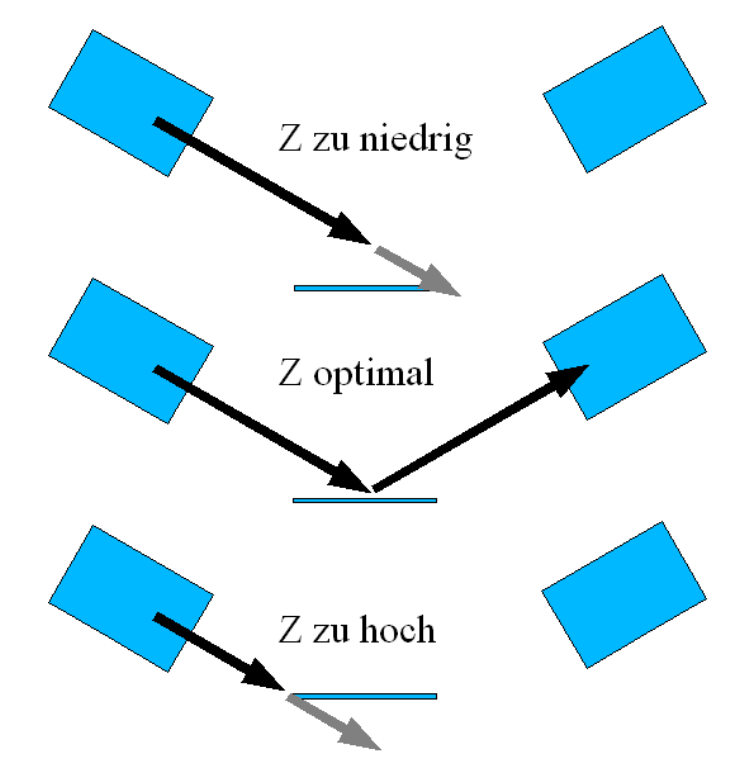
\includegraphics[width = 0.4\textwidth]{pictures/zScan_winkel.png}
            \caption{Die möglichen Geometrien für einen Winkel von $2\theta\neq0°$. Die Mittlere ist die gewünschte Geometrie, bei der die maximale Probenfläche getroffen wird. Entnommen aus \cite{tu_dortmund_versuchsanleitung_2022}}
            \label{fig:zScan_Winkel}
          \end{figure}
      
        \FloatBarrier
        
 
    \subsection{Refelektionsmessung}
        Nach der vorangegangenen Justierung wird ein \textbf{Reflektivitätsscan} durchgeführt, bei dem der Ein- beziehungsweise Ausfallswinkel von Röntgenquelle und Detektor konstant sind, während $2\theta$
        variiert wird. So wird die reflektierte Intensität für verschiedene $2\theta$ und damit verschiedene Impulsüberträge in z-Richtung vermessen. Da es neben der Reflexion auch zu diffuser Streuung kommt,
        muss diese als auftretender Hintergrund vermessenn werden. Dazu wird der Ausfallswinkel des Detektors um 0,1° vom Einfallswinkel der Röntgenröhre variiert $\alpha_{\text{f}} = \alpha_{\text{f}} + 0,1°$
        und ein Scan mit denselben Parametern des Reflektivitätsscans durchgeführt.
    \newpage
    \subsection{Scan-Parameter}
        \FloatBarrier
        \begin{table}[h]
            \centering
            \caption{Die für die verschiedenen Scans verwendeten Parameter. Die z-Position ist nur eine relative Größe zur Justierung und die Einheit daher beliebig. Bearbeitet aus \cite{tu_dortmund_versuchsanleitung_2022}}
            \label{tab:Scan_parameter}
        
            \begin{tabular}{c c c c}
              \toprule
              {Typ} & {Messbereich} & {Schrittweite} & {Messdauer/Messpunkt [s]}\\ 
              \midrule
               Detektorscan  & -0,5° bis 0,5°  & 0,02°  &   1      \\
               z-Scan  & -1 bis 1  & 0,04  &   1      \\
               Rockingscan $2\theta = \SI{0}{\degree}$  & -1° bis 1°  & 0,04°  &   1      \\
               z-Scan  & -0,5 bis 0,5  & 0,02  &   1      \\
               Rockingscan $2\theta = \SI{0.3}{\degree}$  & 0° bis 0,3°  & 0,005°  &   1      \\
               z-Scan $2\theta = \SI{0.3}{\degree}$  & -0,5 bis 0,5  & 0,02  &   1      \\
               Reflektivitätsscan  & 0° bis 2,5°  & 0,005°  &   5      \\
    
              \bottomrule
            \end{tabular}
        \end{table}
        \FloatBarrier



    
    
        
